%%%%%%%%%%%%%%%%%%%% Preamble %%%%%%%%%%%%%%%%%%%%
\documentclass[10pt, paper=a4]{article}
\usepackage{amssymb,amsfonts,amsmath,latexsym,amsthm, mathtools} %mathtext,
\usepackage{booktabs}
\usepackage{multirow}
\usepackage{graphicx}
\usepackage{listings}
\usepackage{chngpage}
\usepackage{cprotect}
\usepackage[font=footnotesize, labelsep=period]{caption}
\usepackage{cite}
\usepackage[scale=0.925]{geometry}
\graphicspath{{images/}}
\usepackage[pdftex,unicode,colorlinks, citecolor=blue,
  filecolor=black, linkcolor=blue, urlcolor=blue]{hyperref}
\usepackage[figure,table]{hypcap}
%%%%%%%%%%%%%%%%%%%% Document %%%%%%%%%%%%%%%%%%%%
\begin{document}
%%%%%%%%%%%%%%%%%%%% Title page %%%%%%%%%%%%%%%%%%%%
\title{Report 02 --- Regression and classification}

\author{Jonathan}

\date{}

\maketitle

\begin{abstract}
We consider linear regression (LR), linear regression with forward
selection (FLR), decision trees (DT), k nearest neighbors (KNN), naive
bayes (NB), artificial neural networks (ANN), and multinomial
regression (MNMR) methods. For regression problem, we found that the
ANN model performs best, and the FLR and the average age (AVE) models
are indistinguishable from each other. For classification problem, we
found the ANN and MNMR to be the best performing models, and showed
them to perform better than the largest class (LCl) classifier and the
linear regression models (LR) using the paired t-test.
  %% Objective: The objective of this second report is to apply the
  %% methods you have learned in the second section of the course on
  %% ”Supervised learning: Classification and regression” in order to
  %% solve both a relevant classification and regression problem for your
  %% data.
\end{abstract}

%%%%%%%%%%%%%%%%%%%% Introduction %%%%%%%%%%%%%%%%%%%%
\section{Regression}
\label{sec:regression}

\subsection{Problem description}
We have selected the regession problem detect spam emails from regular
emails given 57 features.  The features used are wordfrequencies of 54
different words/sings, the amount of capital letters, the longest
sequence of capital letters and the average and the average sequence
of capital letters.

\subsection{Linear Regression with forward selection}
As our dataset has 57 features it is infeasable to compare them all.
Therefore for the for this section only the 12 first features are used.
The 12 features.

Firstly we check if there are any obvious relationships between the
features and if its spam or not. As can be seen there is a difference between the spread for spam
and non spam.

\begin{figure}[h]
  \begin{minipage}{0.3\textwidth}
    a)\\
    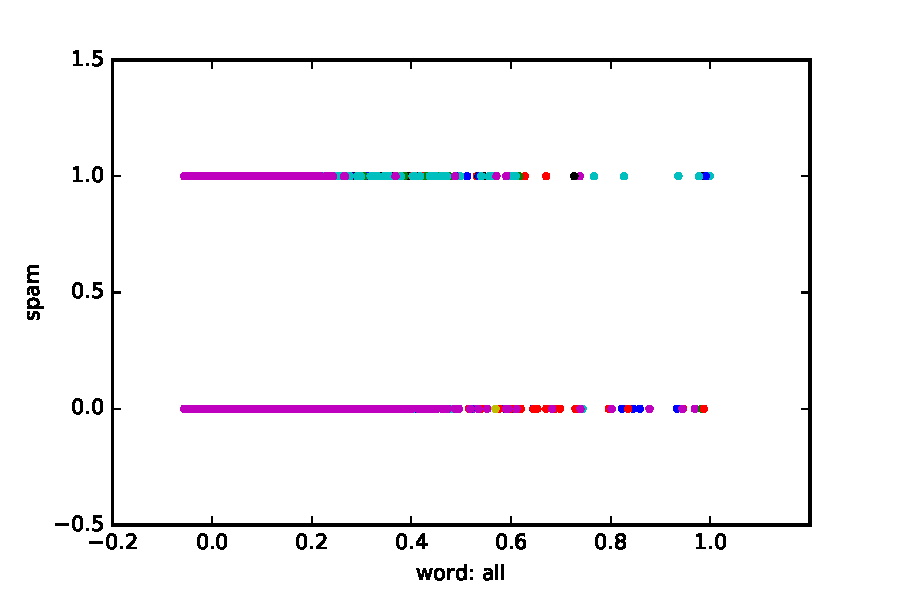
\includegraphics[width = 0.99\textwidth]{../../src/img/all_spam.pdf}
  \end{minipage} \hfill
  \begin{minipage}{0.3\textwidth}
    b)\\
    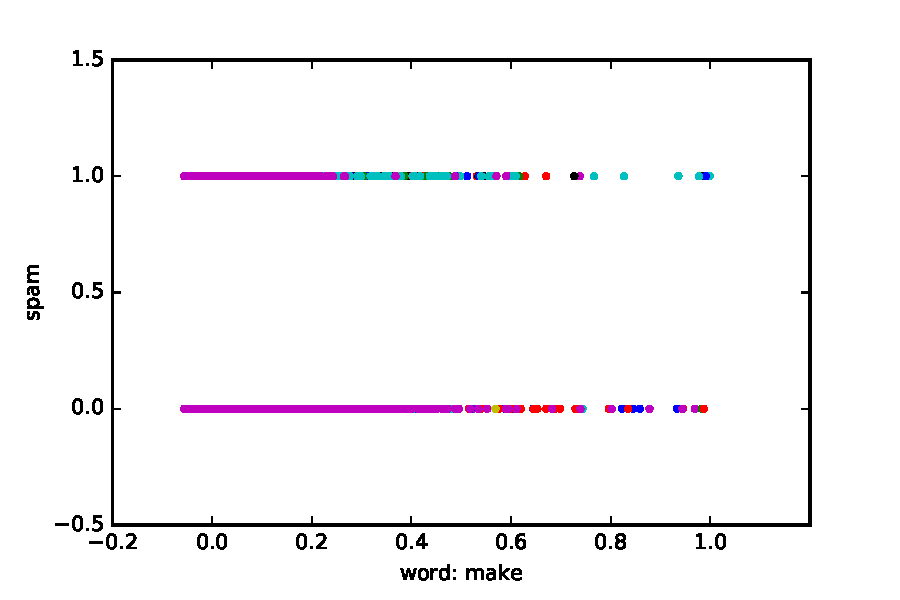
\includegraphics[width = 0.99\textwidth]{../../src/img/make_spam.pdf}
  \end{minipage} \hfill
  \begin{minipage}{0.3\textwidth}
    c)\\
    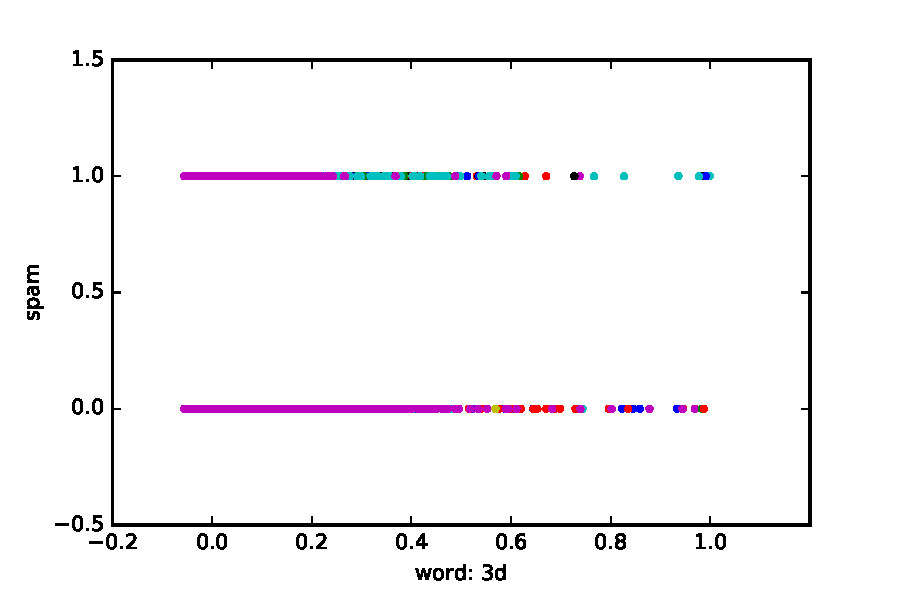
\includegraphics[width = 0.99\textwidth]{../../src/img/3d_spam.pdf}
  \end{minipage} \vfill
  \caption{Spam with some features}
  \label{fig:modelcheck}
\end{figure}

From this we can see that the spam and nonspam is hard to distinguish
just using one feature. But it is possible to see some patter as the
spam is slighly less spread than nonspam.

To figure out what features to use with LR we do forward selection
with a 10-fold cross-validation. Intially this would not run as the 0
feature error is less than any of the features applied to it. To show
that we did it though a inital loss was hardcoded
$loss\_record=[0.27]$.

\begin{figure}[h]
  \centering
  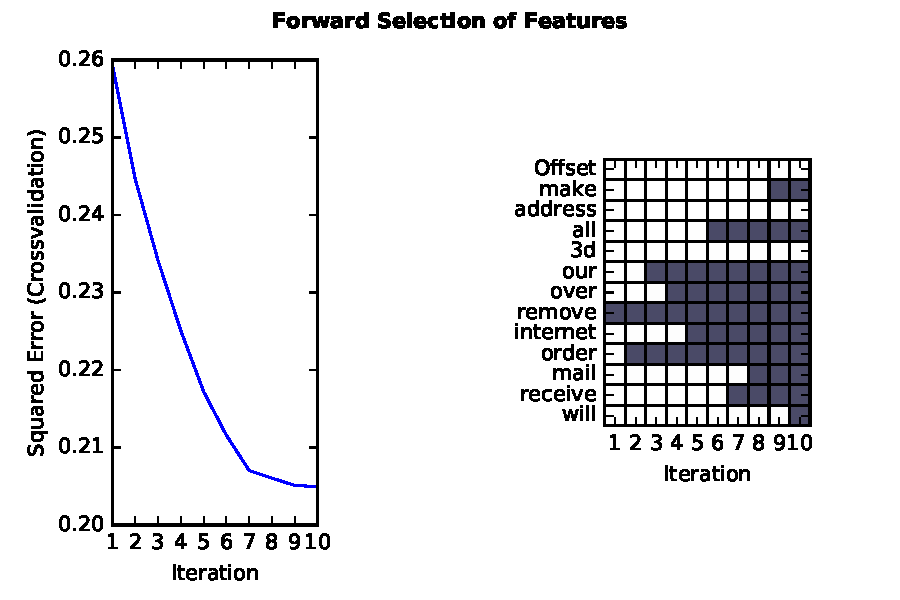
\includegraphics[width = 0.5\textwidth]{../../src/img/best_forward_selection.pdf}
  \caption{Forward selection form 12 features}
  \label{fig:gam}
\end{figure}

This was the best feature selection that LRF could create with 12
features.  If we look at the error rates that are
computed


\begin{Linear regression without feature selection:}{enumerate}
\item Training error: 0.16731688100187755
\item Test error:     0.1690774799900705
\item $R^2$ train:     0.29925175624581624
\item $R^2$ test:     0.2907848014802547
\end{enumerate}


\begin{Linear regression with feature selection:}{enumerate}
\item Training error: 0.1681589246441137
\item Test error:     0.1699619894406495
\item $R^2$ train:     0.2957251509210689
\item $R^2$ test:     0.28707462348598956
\end{enumerate}

We can see that without feature selection we
get a smaller error. From this we can then conclude that Linear
regression will not give us a very good estimator.

\subsection{Data predicitons}
A new email is can now be predicted to be either email or not. This is done by

We can look at the residual error of the blah blah

\begin{figure}[h]
  \centering
  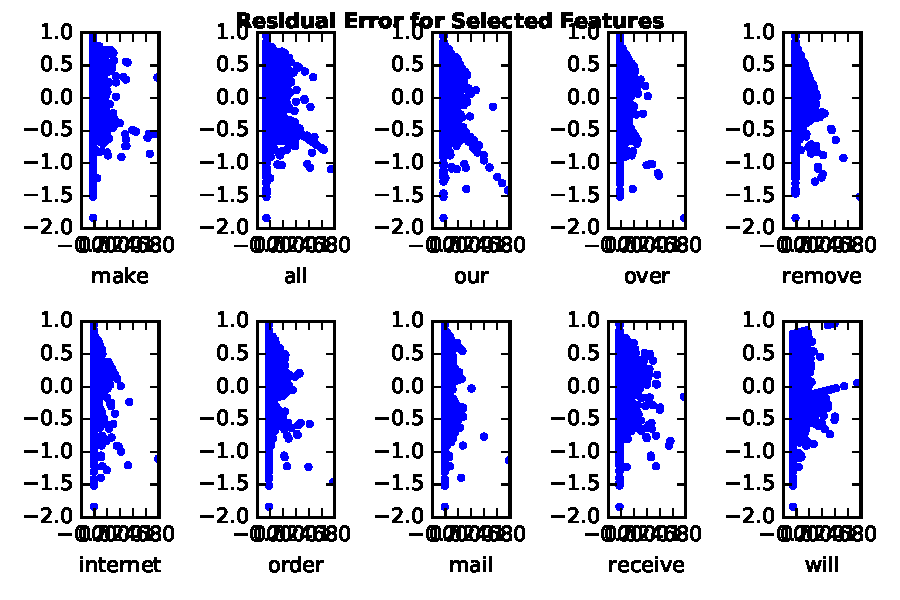
\includegraphics[width = 0.5\textwidth]{../../src/img/residual_error.pdf}
  \caption{Text.}
  \label{fig:gam}
\end{figure}




%%%%%%%%%%%%%%%%%%%% Bibliography %%%%%%%%%%%%%%%%%%%%
\begin{thebibliography}{10}
\bibitem{datadescription} \url{http://archive.ics.uci.edu/ml/datasets/Abalone}
\bibitem{gam} \url{https://en.wikipedia.org/wiki/Generalized_additive_model}
\bibitem{Waugh.thesis} S.~Waugh,''Extending and Benchmark
  Cascade-Correlation,'' Thesis, 1997.
\bibitem{Mayukh} H.~Mayukh, ``Age of Abalones using Physical
  Characteristics: A Classification Problem,'' ECE 539 Fall 2010
  Project Report, Department of Electrical and Computer Engineering
  University of Wisconsin-Madison, 2010.
\end{thebibliography}
\end{document}
